Hallar el área de la región acotada por $y=\tan x$, el eje $x$ y las rectas $x=0$ y $x=\frac{\pi}{3}$.

\nopagebreak
\begin{align*}
\text{Intervalo: } [0, \pi/3]. \quad \Delta x = \frac{\pi}{3n}. \quad x_i = \frac{i\pi}{3n}. \\
\text{Suma de Riemann: } A = \lim_{n \to \infty} \sum_{i=1}^{n} \tan\left(\frac{i\pi}{3n}\right) \frac{\pi}{3n} \\
\text{Evaluando la integral:} \\
A = \int_{0}^{\pi/3} \tan x \, dx = \left[ \ln|\sec x| \right]_{0}^{\pi/3} \\
= \ln(\sec(\pi/3)) - \ln(\sec(0)) \\
= \ln(2) - \ln(1) = \ln 2
\end{align*}

\[
\boxed{\displaystyle \ln 2}
\]

\begin{center}
    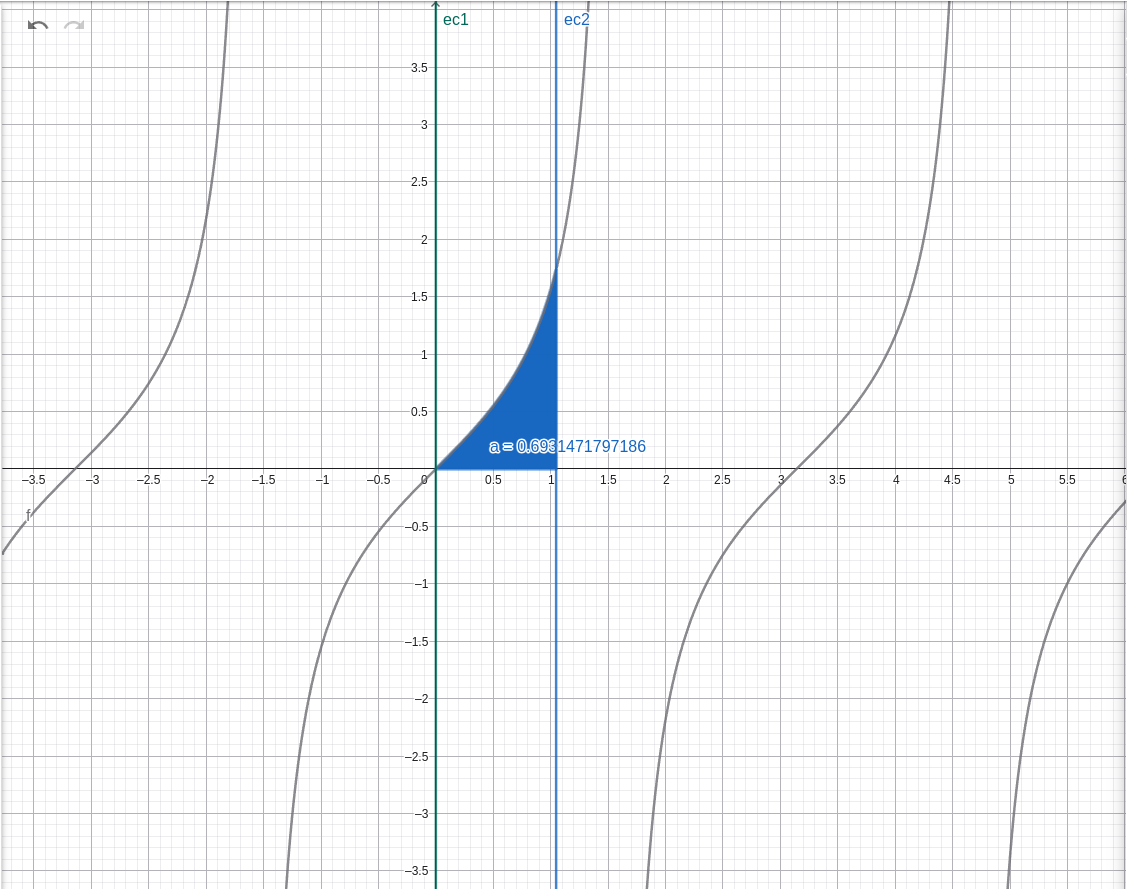
\includegraphics[width=0.5\textwidth]{Graficas/ejer11.png}
\end{center}
